\chapter{Background}\label{s:background}
%\todo{This section provides the necessary context to help the reader understand the remainder of the thesis.}
\section{Problem definition}
One of the main objectives of the Digitale Overheid (Digital Government) is to 'Protect fundamental rights and public values' \cite{DO_agenda}. One could argue protecting the identity and privacy of citizens is part of this objective. The objective of this research is to mitigate the opportunity of identity theft and simultaneously improve citizens’ privacy by making use of appropriate information systems.

\subsection{Grounds for this research}
The Unique Identity Number (UIN) of the Dutch citizen is the ‘Burger Service Nummer’, abbreviated by BSN. In English this means ‘Citizen Service Number’. It’s comparable with the Social Security Number in the USA and it is also being applied to identity a person within Dutch governmental organizations and other parties who are legally permitted to use the BSN. \par
The World Bank \cite{WorldBank_UIN} positions UIN or equivalent ID numbers in the context of "foundational systems". ID numbers are considered to be unique when: firstly, the number-generating process ensures that no two people within the system share the same number and secondly, a deduplication process ensures that the same person does not have multiple identity records or numbers (i.e., that they are unique in the database)." The World Bank identifies two derived strengths, namely ‘Uniqueness and deduplication’ and ‘Data matching and interoperability’. This means each person can be identified uniquely, allowing for a fast and easy exchange of identity related information between different organizations.\par 
However, the benefit of fast and easy exchange of identity related information, is also highly susceptible to misuse. Identity Fraud and Theft leans heavily on the benefit of ‘Data matching and interoperability’ of the UIN. A second form of misuse that leans on this benefit is Unauthorized data correlation. \par
The Dutch governmental audit service, Auditdienst Rijk (ADR) defined gaps and possible improvements in usage of this number\cite{ADR}. This report discusses one of the advantages of BSN being a unique identifier for many different government and non-government organizations. Carrying out their administration more efficiently. Another obtained objective with the introducing of BSN was to prevent identity fraud. Facts and figures in the report of ADR are showing Identity Fraud is growing issue over the last years. A illegally obtained BSN be misused to impact the privacy of citizens negatively while the BSN has advantages within the Dutch government. The same BSN is re-used for different purposes. For example, a bank uses the same BSN of a citizen as a hospital. If the hospital would have a data breach this BSN could be re-used when committing identity fraud, for example at a bank. However, solely having the BSN without other personal information makes identity fraud difficult. At the phase of designing this research the assumption was identity theft was clearly defined and BSN was attribute of personal information to focus on. However, after initiating the research it became clear that a BSN is only a part of the problem and a clear definition of identity theft is needed to prevent different viewpoints of the problem for solution discussions. Together with quantifying and scoping to a operational problem will facilitate discussion on possible and appropriate solutions in information systems. \par

\section{Scope} \label{scope}
To correctly frame the problem and possible solutions it's needed to have clear definitions and scope of this problem. Besides a UIN more attributes of personal identity are linked to an individual person. The 'UK national fraud and cybercrime reporting centre' states a name, date of birth and current or previous addresses could be used to commit identity fraud.\cite{Action_fraud}. This identity data can be obtained in a data breach, for example a breach via commercial parties or (semi-)government. Recent examples are Booking.com \cite{Booking_databreach} or the Dutch GGD \cite{GGD_databreach}.

This section will describe how to frame the position of a UIN among other data within in this domain.
De Vries \etal \cite{Vries2007IdentiteitsfraudeEA} split up identity fraud in two domains: 'Means of identification' (for example a passport or drivers licence) and 'Identity data'. It cannot be denied identity fraud applies on both domains. However, because restrictions in time and resources the scope of this research will be 'Identity data'.
Figure \ref{fig:ID_domain} decomposes the domain of 'Identity data' described by De Vries \etal. This research will narrow it's scope further to 'Formal functional identity data'. 'Profile data' is a value applications of 'Identity data' mainly because a UIN can be used in facilitating combination of data-sets and unauthorized profiling. Definitions provided by De Vries \etal: 
\graphicspath{ {./images/} }
\begin{figure}
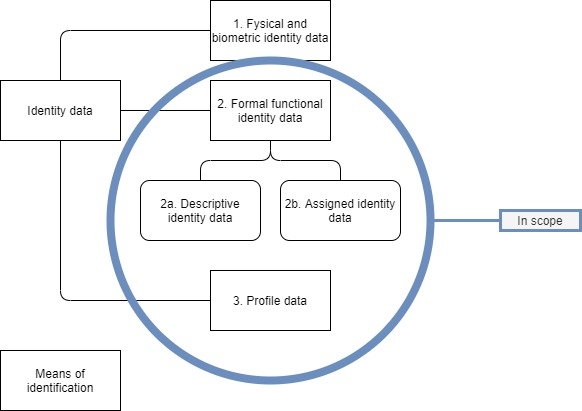
\includegraphics[width=10cm]{Identity data definitions and domain-Overview.jpg}\\
\caption{Domain and scope of Identity Data - De Vries \etal \cite{Vries2007IdentiteitsfraudeEA}}
\label{fig:ID_domain}
\end{figure}
\begin{enumerate}
\item \textit{Physical and bio-metric identity data} - General physically identification data. For example, sex, height, hair color, iris, DNA-profile or medical history
\item \textit{Formal functional identity data} - Data assigned or ascribed in a certain stage of phase of life. To functionally distinguish individuals and assign rights and obligations to this individual.
\begin{enumerate}
\item \textit{Descriptive identity data} - Data that describes a person and the persons surroundings. Information that is close to the individual and is factual and mostly static. For example, family-name, parents, Place, date and time of birth. 
\item \textit{Assigned identity data} - Data that is assigned and mostly describes a (contractual) relationship with organisations to provide products and services.
\end{enumerate}
\item \textit{Profile data} - Based on a certain set of factual data, an algorithm defines profiles that categorize a person. 
\end{enumerate}

\subsection{Definition of Identity Fraud}\label{Def_ID_Fraud}
After commencing this research it became clear Identity Fraud is a catch-all term and a clear definition supports a clear scope. De Vries \etal \cite{97408536fd1c4f4e9d1615b7a4a4473e} have analysed 30 international definitions and formulated a general description "Identity Fraud is to obtain, to possess or to create intentionally, (and) (unlawfully or without consent) false means of identification in order to commit unlawful behaviour, or to have the intention to commit unlawful behaviour." In the footnote it states: "It must be noted that ‘false’ in the description refers to the idea that the means of identification do not identify the person who uses them truthfully." It's needed to say this is a generic definition. Figure \ref{fig:ID_fraud} shows the different types of mismatch between a person and identity data, defined by De Vries \etal \cite{Vries2007IdentiteitsfraudeEA}. The items marked blue in this three define the focus for this research, namely Identity Theft.
\graphicspath{ {./images/} }
\begin{figure}
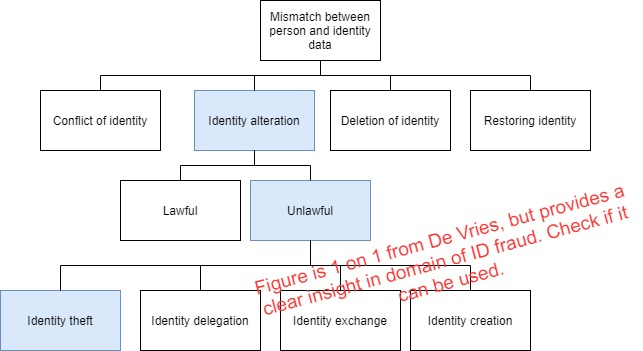
\includegraphics[width=10cm]{Domain of Identity fraud.jpg}\\
\caption{Domain and scope of Identity Fraud - De Vries \etal \cite{Vries2007IdentiteitsfraudeEA}}
\label{fig:ID_fraud}
\end{figure}

\subsection{Quantitative impact of Identity Fraud}\label{QI}
De Vries \etal claim it's difficult to quantify identity fraud because it's incorporated in other crimes\cite{Vries2007IdentiteitsfraudeEA}. Goudriaan \etal claim many crimes in Western countries are not even reported to the police \cite{Gourdriaan_etal}. This research bases quantification of the problem on statistical resources and reports. Quantification is relevant to define problem impact and for purposes of raising awareness and having a generic view on the problem. To quantify impact of solutions it's needed to define methods and probably measuring impact after implementation. Therefore, this is out of scope due to time and capacity restrictions. Impact of possible solutions will be based on logical reasoning and argumentation.

A report of the Auditdienst Rijk (ADR)\cite{ADR} takes in account facts of the 'Citizen service for Identity Fraud' at the 'National Office for Identity Data' (Rijksdienst voor Identiteitsgegevens). Somewhere around 4.000 citizens a year contact this service to report identity fraud. In some cases the impact is low and only a discomfort. In other cases the fraud results in identity theft that can lead to crimes committed by fraudsters in name of that person. Resulting in fines or debts wrongfully matched with the victim.\par 
Statistics Netherlands (CBS) quantified data of identity fraud based on statistical data. Purely looking at the data classified by Identity Fraud, CBS defines it: "Without permission, via internet, making usage of someones personal data for financial gain, for example by withdraw or transfer of money, take out a loan or request of official documents." Roughly 0.5\% of Dutch citizens in 2019 became victim of identity fraud. 0.1\% repeatedly became victim. Based on a population of 17 million, this means roughly 86.000 people are confronted with Identity Fraud each year. 17.000 of them are repeated victims. Figure \ref{fig:CBS_Total_ID_fraud} and Figure \ref{fig:CBS_ID_fraud} show the numbers and how it's divided throughout The Netherlands.

\graphicspath{ {./images/} }
\begin{figure}
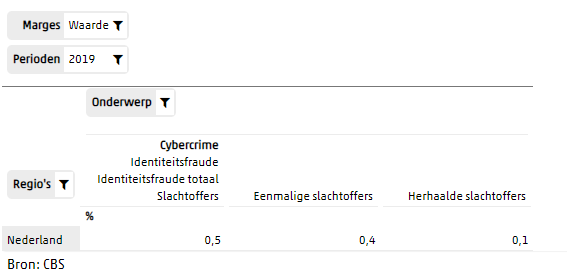
\includegraphics[width=7cm]{Cybercrime - identiteitsfraude Nederland totaal.png}\\
\caption{Victims of Identity Fraud \cite{CBS_IDFraudTable} as a percentage of the total Dutch population in 2019 (17.282.163 \cite{CBS_totalpopulation2019}) - CBS}  
\label{fig:CBS_Total_ID_fraud}
\end{figure}

\graphicspath{ {./images/} }
\begin{figure}
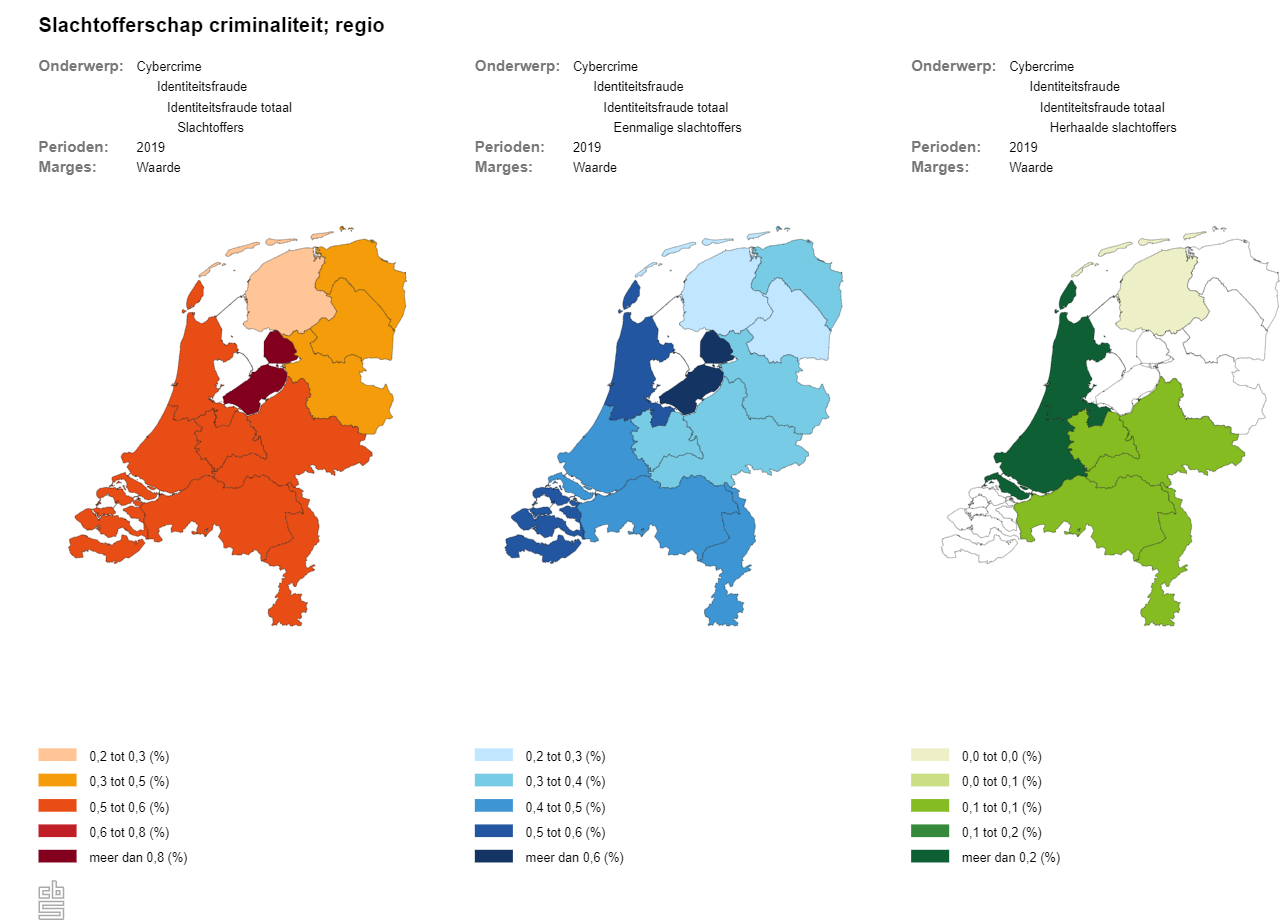
\includegraphics[width=12cm]{Slachtofferschap_delicten__regio__29012022_145152.png}\\
\caption{Division per Province  \cite{CBS_IDFraudTable} - CBS}  
\label{fig:CBS_ID_fraud}
\end{figure}

Another research of the CBS focuses on the impact categorization of victims {\cite{CBS_casualtiesDigitalCrime}}. Concluding property crime is the most victimized crime. 


\subsection{Personal Records Database (BRP) and data provisioning}\label{BRP}
The Dutch Personal Records Database or Basisregistratie Personen (BRP) contains personal information (including BSN) and history of a person in a list of attributes. BRP contains the person lists of both residents and non-resident. Residents are citizens residing in a municipality for a consecutive period. Non-residents are citizens people temporarily living or working within The Netherlands or citizens with Dutch nationality who live abroad. \cite{BRP} The BRP provides a selection of attributes or a complete person list of all attributes to organizations which are permitted by law. Provisioned data is replicated to database managed by that organization. From perspective of data minimization the provided content is minimized for the purpose of use.  
Providing and replicating a set of data should be beheld in the historical perspective of limitations on bandwidth and systems based on batch processing. Currently, bandwidth and real-time processing are not mentioned as concerns by interviewees or consulted experts. It could be considered as a power consumption consideration, but not defined as a quality requirement within this research.

\subsection{Operational problem}\label{OP}
The World Bank ID4ID defines vulnerabilities and risks when UINs are ubiquitous available \cite{WorldBank_protecting}. Identity fraud and unauthorized data correlation are two operational problems. This research will focus on possible practical solutions applied on the BRP focusing on 'Profile data' by using 'Formal functional identity data' as defined in section \ref{Def_ID_Fraud}. UIN and other attributes of a person can be defined as 'Assigned identity data'. Architectural patterns and tactics will be used to help mitigate these problems, taking relevant QA's and ASRs into account. Concretely, providing and replicating identity information could result in unforeseen misuse. Applying patterns to minimize provided data but still providing the lawfully mandated data sharing of BRP could mitigate this risk.
%Dutch laws enforce the exchange of identity data of a citizen and explicitly state to include BSN in this data-set. These laws exist in order to stimulate controlled exchange of personal data. This applies to government bodies , pension providers  and healthcare organizations. Usage of an alternative method, not explicitly providing a BSN, can be interpreted as not complying with these laws. This interpretation is not in scope for my thesis research.\par However, technologies like encryption and pseudonymization are explicitly stated in General Data Protection Regulation (GDPR, REGULATION (EU) 2016/679) {\cite{GDPR}} to be in place as a safeguard. Other rules and regulations may apply, but are not in scope.
%
%\subsection{Pseudonymization or tokenization of a UIN}
%Researching possible solutions in literature and consulting experts showed %two viable methods worth analyzing. Pseudonymization and tokenization. %Pseudonymization of BSN already has been applied within the Dutch %government by Logius. Previous work by AuditDienst Rijk on the usage of BSN % already discussed pseudonymization as an option. Tokenization is an %alternative method largely applied in payment sector (Adyen and Apple Pay) %to ensure privacy of customers. This method is suggested by the World Bank %as a possible solution to replace a UIN, because it’s been applied within %the governments of Austria, India and Estionia.\par
%The difference between these two techniques is mainly the method of %reversing. While pseudonymization needs a key to decrypt, the techniques %behind tokenization need a form of ledger or table to lookup the original %record.
%Off course, there are a lot more technological methods. However, the scope %of this research will not be assessing all of them, rather creating a %useful framework to assess these methods based on requirements.\par
%\textbf{Pseudonymization} 
%GDPR \cite{GDPR} defines ‘pseudonymisation’: means the processing of %personal data in such a manner that the personal data can no longer be %attributed to a specific data subject without the use of additional %information, provided that such additional information is kept separately %and is subject to technical and organisational measures to ensure that the %personal data are not attributed to an identified or identifiable natural %person; \par
%\textbf{Tokenization} is described by The World Bank  as “Tokenization can %protect privacy by ensuring that only tokens, rather than a permanent %identity number or other UIN, are exposed or stored during a transaction.” %Also, by this definition, the same person is represented by different %tokens in different databases. A fundamental property, besides it’s unique %character, is it’s not possible to reverse engineer a person’s identity, %because the unique token does not contain this data.\par
%The World Bank defines two primary types of tokenization. Firstly, %\textbf{Front-end tokenization} is the creation of a token by the user as %part of an online service that can later be used in digital transactions in %place of the original identifier value. Secondly, in case of %\textbf{Back-end tokenization} the identity provider (or token provider) %tokenizes identifiers before they are shared with other systems, limiting %the propagation of the original identifier and controlling the correlation %of data. Back-end tokenization is done automatically by the system without %user intervention, meaning that people do not need to do anything manually %or understand why they would need to create tokens, eliminating any %potential digital divide and protecting identifiers and UIN at source.”